\section{Heap Sort}

\begin{description}
	\item [Heap] Nearly complete binary tree.  All levels, except perhaps the lowest, are complete, and the bottom row is filled from the left.  
	\item [Max-heap property] $A[Parent(i)] \ge A[i]$ The children are no larger than their parent.  
	\item [Min-heap property] $A[Parent(i)] \le A[i]$ The children are no less than their parent.  
\end{description}

\

Max-heap $\{16,14,10,8,7,9,3,2,4,1\}$ as a binary tree.  

\

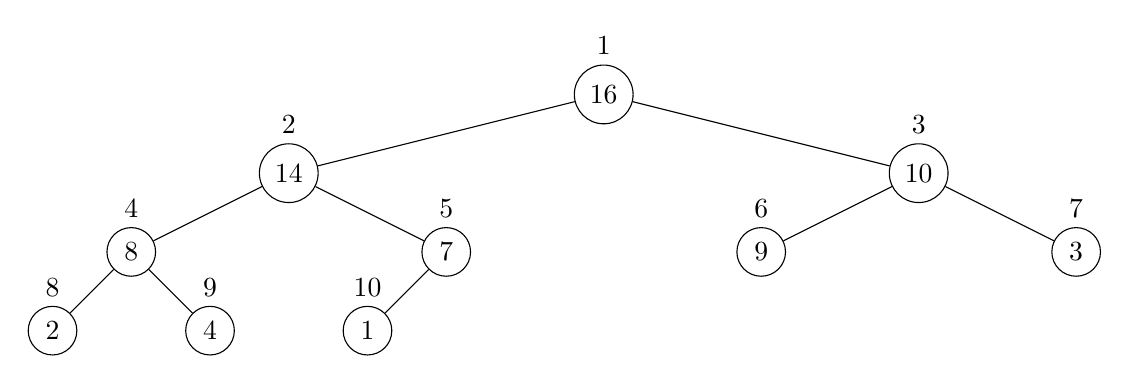
\begin{tikzpicture}[x=10mm, y=10mm]
	\node [circle, draw, label=above:1] (1) at (0,0) {16};
	\node [circle, draw, label=above:2] (2) at (-4,-1) {14};
	\node [circle, draw, label=above:3] (3) at (4,-1) {10};
	\node [circle, draw, label=above:4] (4) at (-6, -2) {8};
	\node [circle, draw, label=above:5] (5) at (-2,-2) {7};
	\node [circle, draw, label=above:6] (6) at (2,-2) {9};
	\node [circle, draw, label=above:7] (7) at (6,-2) {3};
	\node [circle, draw, label=above:8] (8) at (-7,-3) {2};
	\node [circle, draw, label=above:9] (9) at (-5,-3) {4};
	\node [circle, draw, label=above:10] (10) at (-3,-3) {1};
	\foreach \from/\to in {1/2,1/3,2/4,2/5,3/6,3/7,4/8,4/9,5/10}
		\draw (\from) -- (\to);
\end{tikzpicture}

\

Building a max heap takes $O(n)$ time.  

If you have built a max heap and swap out the root node, then it takes $O(\lg n)$ steps to restore the heap.  

Since the head node of a max heap is always the largest node, a method that works to sort the heap is to take out the head node, replace it with the last node, restore the heap, and repeat until the heap is empty.  Since this sort takes $n-1$ steps, and each step takes $O(\lg n)$ time, the sort takes $O(n \lg n)$ time.  

